\documentclass[UTF8]{article}%z指定文档类型
\usepackage[UTF8]{ctex}%显示中文
\usepackage{graphicx}%引用图包
\usepackage{amsfonts,amsmath,amssymb,amstext}%数学相关宏包
\usepackage{color}

\begin{document}%文章开始


\title{网络通信}%文章题目
\maketitle% 显示上述标题信息

\section{Linux基础知识}

\subsection{linux内核}

内核是操作系统的核心,具有很多最基本功能,它负责管理系统的进程、内存、设备驱动程序、文件和网络系统,决定着系统的性能和稳定性。

Linux 内核由如下几部分组成:内存管理、进程管理、设备驱动程序、文件系统和网络管理等。如图所示:

\begin{figure}[htb!]%插入图片
    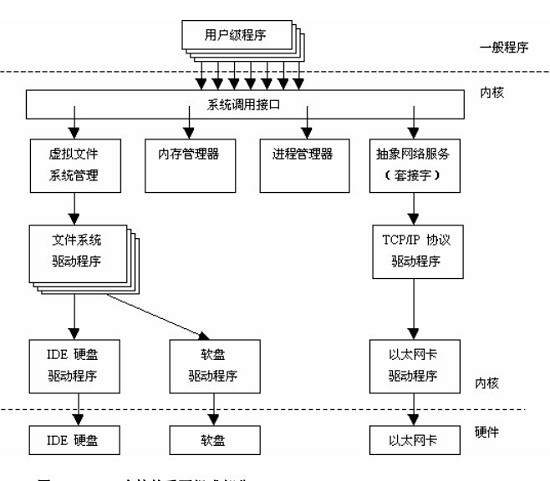
\includegraphics[width=0.8\textwidth]{1.1-1.jpg}
\end{figure}

其中系统调用接口:SCI 层提供了某些机制执行从用户空间到内核的函数调用。

\subsection{Linux 远程登录}

Linux 系统中是通过 ssh 服务实现的远程登录功能,默认 ssh 服务端口号为 22。

安装ssh:yum install ssh

启动ssh:service sshd start

登录远程服务器:ssh -p 50022 my@127.0.0.1

输入密码:my@127.0.0.1:
(-p 后面是端口,my 是服务器用户名,127.0.0.1 是服务器 ip)

回车输入密码即可登录。

\subsection{Linux 进程}

在 Linux 系统中,能够同时运行多个进程,Linux 通过在短的时间间隔内轮流运行这些进程而实现“多任务”。这一短的时间间隔称为“时间片”,让进程轮流运行的方法称为“进程调度” ,完成调度的程序称为调度程序。

Linux 中常见的进程间通讯机制有信号、管道、共享内存、信号量和套接字等。

\subsubsection{相关命令}

可以使用\$ps命令来查询正在运行的进程,比如\$ps -e、-o pid,-o comm,-o cmd,

其中-e表示列出全部进程,-o pid,-o comm,-o cmd分别表示需要PID,COMMAND,CMD信息。

三个信息的意义依次为:PID(process IDentity)是每一个进程的身份(唯一),是一个整数,进程也可以根据PID来识别其他的进程;COMMAND是这个进程的简称;CMD是进程所对应的程序以及运行时所带的参数。

\subsubsection{Linux进程的产生}

当计算机开机的时候,内核(kernel)只建立了一个init进程。Linux内核并不提供直接建立新进程的系统调用。其他所有进程都是init进程通过fork机制建立的。

fork表示:新的进程要通过老的进程复制自身得到,它是一个系统调用。进程存活于内存中。每个进程都在内存中分配有属于自己的一片空间 (address space)。当进程fork的时候,Linux在内存中开辟出一片新的内存空间给新的进程,并将老的进程空间中的内容复制到新的空间中,此后两个进程同时运行。

老进程成为新进程的父进程(parent process),而相应的,新进程就是老的进程的子进程(child process)。一个进程除了有一个PID之外,还会有一个PPID(parent PID)来存储的父进程PID。如果我们循着PPID不断向上追溯的话,总会发现其源头是init进程。所以说,所有的进程也构成一个以init为根的树状结构。

\subsubsection{Linux进程的消失}

当子进程终结时,它会通知父进程,并清空自己所占据的内存,并在内核里留下自己的退出信息(exit code,如果顺利运行,为0;如果有错误或异常状况,为>0的整数)。在这个信息里,会解释该进程为什么退出。

父进程在得知子进程终结时,有责任对该子进程使用wait系统调用。这个wait函数能从内核中取出子进程的退出信息,并清空该信息在内核中所占据的空间。

但是,如果父进程早于子进程终结,子进程就会成为一个孤儿(orphand)进程。孤儿进程会被过继给init进程,init进程也就成了该进程的父进程。init进程负责该子进程终结时调用wait函数。

注意:在Linux中,线程只是一种特殊的进程。多个线程之间可以共享内存空间和IO接口。所以,进程是Linux程序的唯一的实现方式。

\subsection{Linux内存管理}

了让有限的物理内存满足应用程序对内存的大需求量,Linux 采用了称为“虚拟内存”的内存管理方式。Linux 将内存划分为容易处理的“内存页”(对于大部分体系结构来说都是 4KB)。Linux 包括了管理可用内存的方式,以及物理和虚拟映射所使用的硬件机制。

\subsection{Linux文件系统}

Linux系统能支持多种目前流行的文件系统,如EXT2、 EXT3、 FAT、 FAT32、 VFAT和ISO9660。

Linux下面的文件类型主要有:

1) 普通文件:C语言元代码、SHELL脚本、二进制的可执行文件等。分为纯文本和二进制;

2) 目录文件:目录,存储文件的唯一地方;

3) 链接文件:指向同一个文件或目录的的文件;

4) 设备文件:与系统外设相关的,通常在/dev下面。分为块设备和字符设备;

5)管道(FIFO)文件: 提供进程之间通信的一种方式;

6)套接字(socket) 文件: 该文件类型与网络通信有关;

可参考:https://www.linuxprobe.com/linux-system-structure.html

\subsection{Linux防火墙}

\subsubsection{常用命令}

\begin{itemize}
    \item 启动:systemctl start firewalld
    \item 重启:systemctl restart firewalld
    \item 停止:systemctl stop firewalld
    \item 重新加载:firewall-cmd --reload
    \item 查看firewalld的运行状态:
    
        firewall-cmd --state

    \item 取消开放https服务,即禁止https服务:
    
        firewall-cmd --zone=drop --remove-service=https

    \item 开放22端口:
    
        firewall-cmd --zone=drop --add-port=22/tcp

    \item 取消开放22端口:
    
        firewall-cmd --zone=drop --remove-port=22/tcp

    \item 开放两个端口:
    
    firewall-cmd --zone=drop --add-port=8080-8081/tcp

    \item 查询drop区域开放了哪些端口:
    
    firewall-cmd --zone=drop --list-ports

    \item 其他常用命令:
    
    允许icmp协议流量,即允许ping:

    firewall-cmd --zone=drop --add-protocol=icmp

    取消允许icmp协议的流量,即禁ping:

    firewall-cmd --zone=drop --remove-protocol=icmp
    
    查询drop区域开放了哪些协议:

    firewall-cmd --zone=drop --list-protocols

    将原本访问本机888端口的流量转发到本机22端口:
    
    firewall-cmd --zone=drop --add-forward-port
    =port=888:proto=tcp:toport=22
\end{itemize}


\section{socket基础}

\subsection{socket通信的概念}

套接字,运行在计算机中的两个程序通过socket建立起一个通道,数据在通道中传输。套接字可以看成是两个网络应用程序进行通信时,各自通信连接中的端点,这是一个逻辑上的概念。它是网络环境中进程间通信的API(应用程序编程接口)(是IP地址和端口结合)。

socket把复杂的TCP/IP协议族隐藏了起来,只要用好socket相关的函数,就可以完成网络通信。

\subsection{socket的分类}

socket提供了流(stream)和数据报(datagram)两种通信机制,即流socket和数据报socket。

流socket基于TCP协议,是一个有序、可靠、双向字节流的通道,传输数据不会丢失、不会重复、顺序也不会错乱。类似于打电话。

数据报socket基于UDP协议,不需要建立和维持连接,可能会丢失或错乱。UDP不是一个可靠的协议,对数据的长度有限制,但是它的速度比较高。类似于短信。

在实际开发中,数据报socket的应用场景极少。

\subsection{socket通信的过程}

\subsubsection{服务端}

\begin{itemize}
    \item 创建服务端的socket。socket()
    \item 把服务端指定的用于通信的ip地址和端口绑定到socket上。bind()
    \item 把socket设置为监听模式,以监听用户请求。listen()
    \item 接受客户端的连接。accept()
    \item 与客户端通信,接收客户端发过来的报文后,回复处理结果。send()/recv()
    \item 不断的重复上一步步,直到客户端断开连接。
    \item 关闭socket,释放资源。close()
\end{itemize}

\subsubsection{客户端}

\begin{itemize}
    \item 创建客户端的socket。socket()
    \item 向服务器发起连接请求。connect()
    \item 与服务端通信,发送一个报文后等待回复,然后再发下一个报文。send()/recv()
    \item 不断的重复上一步,直到全部的数据被发送完。
    \item 关闭socket,释放资源。close()
\end{itemize}

\begin{figure}[htb!]%插入图片
    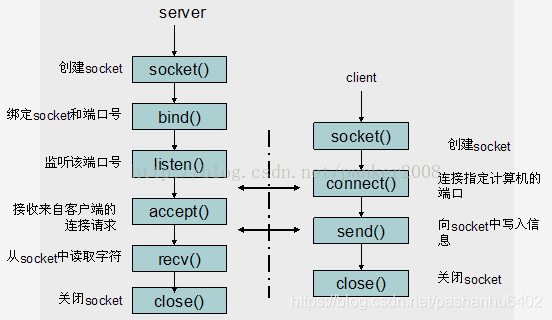
\includegraphics[width=0.8\textwidth]{2.3-1.png}
\end{figure}

\subsection{Socket}

在Linux系统中,一切输入输出设备皆文件。而socket本质上可以视为一种特殊的文件,即通信的实现,因此socket的通信过程也可以理解为通过“打开open –> 读写write/read –> 关闭close”模式的操作过程。

注意:

a. 客户端有一个socket,是用于发送报文的socket;而服务端有两个socket,一个是用于监听的socket,还有一个就是客户端连接成功后,由accept函数创建的用于与客户端收发报文的socket。

b. socket是系统资源,操作系统打开的socket数量是有限的,在程序退出之前必须关闭已打开的socket,就像关闭文件指针一样,就像delete已分配的内存一样,极其重要。

c. 关闭socket的代码不能只在main函数的最后,那是程序运行的理想状态,还应该在main函数的每个return之前关闭。

d. socket类型的servaddr的地址,(struct sockaddr *)\&servaddr。

\subsection{客户端服务端主要参数及结构体}

\subsubsection{socket()返回的值}

返回值称为socket描述符(socket descriptor),其本质是一个文件描述符,是一个整数。把它作为参数,通过它来进行一些读写操作。

0表示标准输入,1表示标准输出,2表示标准错误。

注意:默认创建的socket是主动连接的。

\subsubsection{有关定义}

\begin{itemize}
    \item 大端模式、小端模式:“大端”和”小端”表示多字节值的哪一端存储在该值的起始地址处;小端存储在起始地址处,即是小端字节序;大端存储在起始地址处,即是大端字节序。
    
    a. 大端字节序(Big Endian):最高有效位存于最低内存地址处,最低有效位存于最高内存处;
   
    b. 小端字节序(Little Endian):最高有效位存于最高内存地址,最低有效位存于最低内存处。

    \item 网络字节序NBO:网络字节序是大端字节序。在进行网络传输的时候,发送端发送的第一个字节是高位字节。
    \item 主机字节序HBO:不同的机器HBO不相同,与CPU的设计有关,数据的顺序是由CPU决定的,而与操作系统无关。不同体系结构的机器之间不能直接通信,所以要转换成一种约定的顺序,也就是网络字节顺序。存在专门的函数来进行二者的转换。
    \item 命名规则:
    
    socket字符:sockfd客户端,listenfd服务端;

    网络地址:clientaddr客户端,servaddr服务端;
    \item 

\end{itemize}

\subsubsection{struct hostent* h}

域名和网络地址结构体:

struct hostent

\{

\qquad    char *h\_name;  //主机名,即官方域名
    
\qquad    char **h\_aliases;  //主机所有别名构成的字符串数组,同一IP可绑定多个域名

\qquad    int h\_addrtype; //主机IP地址的类型,例如IPV4(AF\_INET)还是IPV6【需转化】

\qquad    int h\_length;  //主机IP地址长度,IPV4地址为4,IPV6地址则为16。【常用】

\qquad    char **h\_addr\_list;  //主机的ip地址,虽然为char形式,但以网络字节序格式存储。若要打印出这个IP,需要调用inet\_ntoa()。【常用】

\};

注意:
a. 通常用于客户端已知对方ip情况下获得对方网络其他信息。

b. 与下面的结构体一样,定义时指的是哪个端,其内数据就指哪个端。

\paragraph{操作函数}~{}


\begin{itemize}
    \item *gethostbyname(const char *name);
    
    用于客户端指定服务端的ip地址,详见后文函数介绍,注意参数为char类型的常量。成功执行该函数后结构体内各变量均可获得。

    \item inet\_ntop(h->h\_addrtype);
    
    将网络字节序的二进制转换为文本字符串的格式。

\end{itemize}

\subsubsection{struct sockaddr\_in servaddr}

表示地址信息的数据结构(体),存放了目标地址和端口。与结构体sockaddr把目标地址和端口信息混在一起了不同,其把port和addr 分开储存在两个变量中。

struct sockaddr\_in

\{

\qquad sa\_family\_t \quad sin\_family; //协议族,在socket编程中只能是AF\_INET。

\qquad unit16\_t \quad sin\_port; //16位的TCP/UDP端口号。

\qquad struct in\_addr \quad sin\_addr; //32位IP地址

\qquad char \quad sin\_zero[8]; //不使用。

\}

其中:

struct in\_addr 

\{

\qquad in\_addr\_t s\_addr; //32位IP v4地址。

\qquad (可表示为:servaddr.sin\_addr.s\_addr)

\}

\paragraph{操作函数}~{}

\begin{itemize}
    \item inet\_addr():将网络地址字符串(IP字符串)转为网络二进制数字(网络字节序),返回的IP地址是网络字节序的。
    
    (const char----> in\_addr\_t)(ascii to network)

    \item inet\_ntoa():将网络二进制数字(网络字节序)转为网络地址字符串(IP字符串)。
    
    (in\_addr\_t---->const char)(network to ascii)


    \item inet\_aton():将网络地址转为网络字节序,与inet\_addr的区别是,结果不是作为返回值,而是保存形参inp所指的in\_addr\_t结构体中。函数原型:int inet\_aton(cont char* cp, struct in\_addr\_t *inp)
    
    (const char----> in\_addr\_t)(ascii to network)

    \item htons()作用是将端口号由主机字节序转换为网络字节序的整数值。
    
    (int to in\_addr\_t)(host to net)
    
    (不一定是in\_addr\_t,满足要求的字符即可,例如unit16\_t)

    \item htonl()作用和htons()一样,不过它针对的是32位的(long),而htons()针对的是16位的(short)。
    
    (host to net)

    \item 与htonl()和htons()作用相反的两个函数是:ntohl()和ntohs()。
    
    (net to host)
    
    \item 应用:服务端绑定(自身的)IP地址:

    servaddr.sin\_addr.s\_addr = \textcolor{red}{inet\_addr}("192.168.149.129");  // 指定ip地址  
    
    servaddr.sin\_addr.s\_addr = \textcolor{red}{htonl(INADDR\_ANY)};  // 本主机的任意ip地址。在实际开发中,采用任意ip地址的方式比较多。

    \item 应用:服务端绑定通信端口,也可用于客户端指定服务端的通信端口:
    
    servaddr.sin\_port = \textcolor{red}{htons}(5000);  // 通信端口5000

    \item 注意htons()的参数为int型的无符号短整形数,若用argv[]来传递,需要强制转换类型函数atoi()。同理htonl()。

    \item 注意:不论是那个端的程序采用,servaddr指的是哪个端,端口、IP地址就是哪个端。

\end{itemize}

注意:通常服务器在启动的时候都会绑定一个众所周知的地址(如ip地址+端口号),用于提供服务,客户就可以通过它来接连服务器;而客户端就不用指定,有系统自动分配一个端口号和自身的ip地址组合。这就是为什么通常服务器端在listen之前会调用bind(),而客户端就不会调用,而是在connect()时由系统随机生成一个。

\subsection{客户端服务端函数}

以下为几种常用的接口函数:

\subsubsection{socket()函数}

功能:用于创建一个新的socket。对应于普通文件的打开操作。

返回值:成功则返回一个socket描述符,失败返回-1,错误原因存于errno 中。

使用范围:客户端、服务端。

\paragraph{函数声明}~{}

int socket (int domain, int type, int protocol);

\begin{itemize}
    \item domain:协议域,又称协议族(family)。协议族决定了socket的地址类型,在通信中必须采用对应的地址。
    
        AF\_INET:决定了要用ipv4地址(32位的)与端口号(16位的)的组合;

        AF\_UNIX:决定了要用一个绝对路径名作为地址。

    \item type:指定socket类型。
    
        流式socket(SOCK\_STREAM)是一种面向连接的socket,针对于面向连接的TCP服务应用。数据报式socket(SOCK\_DGRAM)是一种无连接的socket,对应于无连接的UDP服务应用。

    \item protocol:指定协议。
    
        常用协议有IPPROTO\_TCP、IPPROTO\_UDP、IPPROTO\_STCP、IPPROTO\_TIPC等,分别对应TCP传输协议、UDP传输协议、STCP传输协议、TIPC传输协议。

        注意为0则与type相匹配,与type不能随意匹配。

    \item 正常情况,第一个参数只能填AF\_INET,第二个参数只能填SOCK\_STREAM,第三个参数只能填0。
\end{itemize}

使用:\textcolor{red}{int sockfd = socket(AF\_INET,SOCK\_STREAM,0))}

\subsubsection{send()函数}

功能:用于把数据通过socket发送给对端。

返回值:函数返回已发送的字符数。出错时返回-1,错误信息errno被标记。

适用范围:客户端、服务端。

注意:注意,就算是网络断开,或socket已被对端关闭,send函数不会立即报错,要过几秒才会报错。如果send函数返回的错误(<=0),表示通信链路已不可用。

\paragraph{函数声明}~{}

ssize\_t send(int sockfd, const void *buf, size\_t len, int flags);

sockfd:为已建立好连接的对方端的socket。

buf:为需要发送的数据的内存地址,可以是C语言基本数据类型变量的地址,也可以数组、结构体、字符串,内存中有什么就发送什么。

len:需要发送的数据的长度,为buf中有效数据的长度。

flags:填0, 其他数值意义不大。

使用:\textcolor{red}{iret=send(sockfd,buffer,strlen(buffer),0);}

\subsubsection{recv()函数}

功能:用于接收对方socket发送过来的数据。

返回值:函数返回已接收的字符数。出错时返回-1,失败时不会设置errno的值。

适用范围:客户端、服务端。

注意:如果socket的对端没有发送数据,recv函数就会等待,如果对端发送了数据,函数返回接收到的字符数。出错时返回-1。如果socket被对端关闭,返回值为0。如果recv函数返回的错误(<=0),表示通信通道已不可用。

\paragraph{函数声明}~{}

ssize\_t recv(int sockfd, void *buf, size\_t len, int flags);

sockfd:为已建立好连接的对方端的socket。

buf:为用于接收数据的内存地址,可以是C语言基本数据类型变量的地址,也可以数组、结构体、字符串,只要是一块内存就行了。

len:需要接收数据的长度,不能超过buf的大小,否则内存溢出。

flags:填0, 其他数值意义不大。

使用:\textcolor{red}{iret=recv(sockfd,buffer,sizeof(buffer),0);}

\subsubsection{gethostbyname()函数}

功能:把ip地址或域名转换为hostent 结构体表达的地址。

返回值:如果成功,返回一个hostent结构指针,失败返回NULL。

适用范围:客户端。

注意:只要地址格式没错,一般不会返回错误。失败时不会设置errno的值。

\paragraph{函数声明}~{}

struct hostent *gethostbyname(const char *name);

name:域名或者主机名,例如"192.168.1.3"、"www.freecplus.net"等。

使用:\textcolor{red}{struct hostent *h = gethostbyname(argv[1])}

\subsubsection{附注:memset()函数}

void *memset(void *str, int c, size\_t n)

str -- 指向要填充的内存块。

c -- 要被设置的值。该值以 int 形式传递,但是函数在填充内存块时是使用该值的无符号字符形式。默认0。

n -- 大小,sizeof(str)。

注意:与malloc不同之处为后者未初始化。而new 返回指定类型的指针,并且可以自动计算所需要大小。

\subsubsection{附注:memcpy()函数}

void *memcpy(void *str1, const void *str2, size\_t n)

str1 -- 指向用于存储复制内容的目标数组,类型强制转换为 void* 指针。

str2 -- 指向要复制的数据源,类型强制转换为 void* 指针。

n -- 要被复制的字节数。

\subsubsection{connect()函数}

功能:客户端通过调用connect函数来建立客户端socket与服务器的连接。

返回值:成功则返回0,失败返回-1,错误原因存于errno 中。

适用范围:客户端。

注意:如果服务端的地址错了,或端口错了,或服务端没有启动,connect一定会失败。

\paragraph{函数声明}~{}

int connect(int sockfd, const struct sockaddr *addr, socklen\_t addrlen);

sockfd:客户端的socket描述字。

*addr:服务端的socket地址信息。

addrlen:服务端socket地址的长度(addr结构体的大小)。

使用:\textcolor{red}{connect(sockfd, (struct sockaddr *)\&servaddr,sizeof(servaddr))}

\subsubsection{bind()函数}

功能:服务端把自身用于通信的地址和端口绑定到socket上。

返回值:成功则返回0,失败返回-1,错误原因存于errno 中。

适用范围:服务端。

注意:如果绑定的地址错误,或端口已被占用,bind函数一定会报错,否则一般不会返回错误。

\paragraph{函数声明}~{}

int bind(int sockfd, const struct sockaddr *addr, socklen\_t addrlen);

sockfd:服务端socket。

*addr:服务端的socket地址信息。(一个const struct sockaddr *指针,指向要绑定给sockfd的协议地址。存放了服务端用于通信的地址和端口。)

addrlen:服务端socket地址的长度。

使用:\textcolor{red}{bind(listenfd,(struct sockaddr *)\&servaddr,sizeof(servaddr));}

注意调用时参数使用强制类型转换。

\subsubsection{listen()函数}

功能:用于把主动连接socket变为被动连接的socket,使得这个socket可以接受其它socket的连接请求,从而成为一个服务端的socket。 当调用listen之后,服务端的socket就可以调用accept来接受客户端的连接请求。

返回值:0-成功, -1-失败,错误原因存于errno 中。

listen函数一般不会返回错误。

适用范围:服务端。

\paragraph{函数声明}~{}

int listen(int sockfd, int backlog);

sockfd:是服务端已经被bind过的socket。

backlog:这个参数涉及到一些网络的细节,比较麻烦,填5、10都行,一般不超过30。

使用:\textcolor{red}{listen(listenfd,5);}

\subsubsection{accept()函数}

功能:用于服务端接受客户端的连接。

返回值:成功则返回0,失败返回-1,错误原因存于errno 中。

适用范围:服务端。

注意:

a. accept在等待的过程中,如果被中断或其它的原因,函数返回-1,表示失败,如果失败,可以重新accept。

b. accept函数等待客户端的连接,如果没有客户端连上来,它就一直等待,这种方式称之为阻塞。

c. accept等待到客户端的连接后,\textcolor{red}{创建一个新的socket,函数返回值就是这个新的socket,服务端使用这个新的socket和客户端进行报文的收发。}

\paragraph{函数声明}~{}

int accept(int sockfd,struct sockaddr *addr,socklen\_t *addrlen);

sockfd:是服务端已经被listen过的socket。

addr:用于存放客户端的地址信息,用sockaddr结构体表达,如果不需要客户端的地址,可以填0。也可以先定义一个空的客户端地址,然后填进去。

addrlen:用于存放addr参数的长度,如果addr为0,addrlen也填0。

使用:\textcolor{red}{clientfd=accept(listenfd,(struct sockaddr *)\&clientaddr,(socklen\_t*)\&socklen);}

\subsection{注意事项}

\begin{itemize}
    \item 每一个端,具有一个socket指示符、一个地址信息。
    \item 凡是函数参数含有地址信息的,均需要强制格式化:
    
    (struct sockaddr *)\& + 地址名

    \item 
\end{itemize}

\section{}




\begin{itemize}
    \item 
    \item 
    \item 
\end{itemize}

\end{document}%文章结束
